\chapter{Bottom up parser}

Il \textbf{parser bottom up} è un tipo di analizzatore sintattico che che costruisce l'albero di derivazione partendo dalle foglie, viene anche detto \textbf{Shift-Reduce} in quanto possiede due operazioni fondamentali:
\begin{itemize}
    \item \texttt{Shift}: un simbolo terminale viene spostato dall'input alla pila 
    \item \texttt{Reduce}: una serie di simboli (terminali e non terminali) sulla cima della pila corrisponde al "reverse" di una parte destra di una produzione, ovvero:
    \[
        A\to\alpha \in R - \alpha^R \text{ sulla pila}
    \]
    La stringa $\alpha^T$ viene rimossa dalla pila e sostituita con $A$, quindi $\alpha$ viene ridotta ad $A$
\end{itemize}

Possono essere di diversi tipi

\section{Parser shift-reduce nondeterministico}
\begin{algorithm}
    \caption{Parser shift-reduce nondeterministico}
    \KwIn{Una grammatica libera $G$ con simbolo iniziale $S$ e una stringa $w\in T^*$}
    \KwOut{Una stringa $w\in T^*$}

    Inizializziamo la pila a $\$$\;
    Inizializziamo l'input con $w\$$\;
    usaimo il $PDA$ seguente per trovare la derivazione per $w\$$:
    \[
        M=(T, \{q\},\underbracket{T\cup NT \cup \{\$\}}_{\Gamma: \text{ovvero i simboli sulla pila}}, \delta, \varnothing)
    \]
    Dove:
    \begin{enumerate}
        \item $(q,aX)\in \delta (q,a,X)\forall A\in T\forall X\Gamma\quad \text{SHIFT}$
        \item $(q,A)\in\delta(q,\epsilon, \alpha^R)$ se $A\in \alpha\in R\quad \text{REDUCE}$
        \item $(q,\epsilon)\in \delta(q,\$,S\$)\quad \text{accept}$
    \end{enumerate}\;
    ogni volta che facciamo "reduce", forniamo in output la produzione usata\;
    alla fine, $S\$$ sulla pila, con $\$$ in input $\implies$ accettiamo\;
\end{algorithm}

\nt{
    generalizzazione della def. di $PDA$ dove non si consuma solo il top della pila, ma una serie di caratteri contigui a caminciare dal top
}

\esempio{
    Sia la seguente grammatica
    \[
        \begin{array}{l}
            E\to T\mid T+E \mid T-E\\
            T\to A\mid A*T\\
            A\to a\mid b\mid (E)
        \end{array}
    \]
    \[
        \begin{array}{|c|l|l|l|l|}
        \hline
        \textbf{N.} & \textbf{Pila} & \textbf{Input} & \textbf{Azione} & \textbf{Output} \\ \hline
        1  & \$                  & a+b*b\$              & Shift         &                 \\ \hline
        2  & \$a                & +b*b\$               & Reduce        & A \to a         \\ \hline
        3  & \$A                & +b*b\$               & Reduce        & T \to A         \\ \hline
        4  & \$T                & +b*b\$               & Shift         &                 \\ \hline
        5  & \$T+               & b*b\$                & Shift         &                 \\ \hline
        6  & \$T+b              & *b\$                 & Reduce        & A \to b         \\ \hline
        7  & \$T+A              & *b\$                 & Shift         &                 \\ \hline
        8  & \$T+A*             & b\$                  & Shift         &                 \\ \hline
        9  & \$T+A*b            & \$                   & Reduce        & A \to b         \\ \hline
        10 & \$T+A*B            & \$                   & Reduce        & T \to A * T     \\ \hline
        11 & \$T+A*T            & \$                   & Reduce        & E \to T + T     \\ \hline
        12 & \$E                & \$                   & Reduce        & E \to T + T     \\ \hline
        13 & \$E                & \$                   & Accept        &                 \\ \hline
        \end{array}
    \]

    Si ha che:
    \[
        E\implies T+E\implies T+T \implies T + A* T \implies T+A*A \implies T + A * b \implies T + b * b \implies A + b*b  \implies a + b*b
    \]

    Il cui albero è:
    \begin{center}
        \begin{tikzpicture}
            \Tree [
                .E
                [
                    .T
                    [
                        .A
                        [
                            .a
                        ]
                    ]
                ]
                [
                    .+
                ]
                [
                    .E
                    [
                        .T
                        [
                            .A
                            [
                                .b
                            ]
                        ]
                        [
                            .*
                        ]
                        [
                            .T
                            [
                                .A
                                [
                                    .b
                                ]
                            ]
                        ]
                    ]
                ]
            ]
        \end{tikzpicture}
    \end{center}
    
    Le cui proprietà sono:
    \begin{center}
        \item Costruzione dell'albero di derivazione \textit{bottom-up}    
        \item Derivazione canonica a destra a rovescio
        \item forte non-determinismo:
        \begin{itemize}
            \item \textbf{conflitti shift-reduce}:
            \begin{itemize}
                \item $\$a \quad +b*b\$ \quad \text{shift}$
                \item $\$ a+ \quad b*b \$$
            \end{itemize}
            \item \textbf{Conflitti reduce-reduce}
            \begin{itemize}
                \item $\$T+A*T\quad\$$ reduce $E\to T$
                \item $\$T+A*E\quad\$$
            \end{itemize}
        \end{itemize}
    \end{center}
}

\nt{Si noti quindi che questo tipo parser genera moltissimi confilitti, in diverse sistuazioni era appunto possibile scegliere strade che non portano a riconoscere la stringa. F}

Per "risolvere" tale nondeterminismo occorre fornire al PDA una tabella parsing (struttura di controllo) che "aiuti" a scegliere l'azione giusta, ed è grazie all'uso di questa che nascono i cosiddetti \textbf{parser LR}

\section{Parser LR}
\dfn{Parser LR}{
    Il \textbf{parser LR} è un tipo di analizzatore sintattico che utilizza un approccio bottom-up per analizzare un input e verificare se appartiene al linguaggio generato da una grammatica libera. Il termine LR indica che:
    \begin{itemize}
        \item L: sta per \textit{left-to-right}: l'analisi dell'input avviene da sinistra a destra
        \item R: sta per \textit{Rightmost derivation}: l'analisi ricostruisce una derivazione più a destra in senso inverso
    \end{itemize}
}

Presento, qui uno schema bellino bellino:

%TODO DA FARE QUESTA GIGAMINCHIATA
\begin{center}
    \begin{tikzpicture}
        % Input
        \node at (-2.5, 3.5) {Input:};
        \node[stack] (input1) at (-1,0) {$a_1$};
        \node[stack, right of=input1] (input2) {$a_2$};



        % \node[stack] (input2) at (0,1) {$a_2$};
        % \node[stack] (dots) at (1, 2) {$\dots$};
        % \node[stack] (inputn) at (2,3) {$a_i$};
        % \node[stack] (end) at (3, 4) {$\dots$};
        % \node[stack] (end) at (4, 5) {$a_k$};
        % \node[stack] (end) at (5, 6) {$\$$};
    
        % Parser LR block
        \node[block] (parserLR) at (0,1.5) {Parser LR};
    
        % Output
        \node at (4.5, 1.5) {Output:};
        \node[align=center] (output) at (6.7,1.5) {Derivazione \\ \textit{rightmost} \\ = albero di derivazione};
    
        % Parsing Table
        \node[block] (table) at (0,-1.5) {Tabella di Parsing $M$ \\ \vspace{0.2cm} \textbf{Azione} (Shift/Reduce) \\ sui Terminali \\ \textbf{GOTO} sui Nonterminali};
    
        % Stack
        \node at (-4.2, 1.5) {Pila:};
        \node[stack] (stack0) at (-3.5,1.5) {$S_0$};
        \node[stack] (stackdots) at (-3.5,0.7) {$\vdots$};
        \node[stack] (stackn) at (-3.5,-0.1) {$S_m$};
    
        \node at (-4.2, -1.5) {Pila simboli:};
        \node[stack] (symbol0) at (-3.5,-1.5) {$X_0$};
        \node[stack] (symboldots) at (-3.5,-2.3) {$\vdots$};
        \node[stack] (symboln) at (-3.5,-3.1) {$X_m$};
    
        % Arrows
        \draw[arrow] (input1.south) -- (parserLR.north);
        \draw[arrow] (parserLR.south) -- (table.north) node[midway,right] {consulta};
        \draw[arrow] (parserLR.east) -- (output.west);
    
        \draw[arrow] (stack0.east) ++(0.2,0) -- (parserLR.west);
        \draw[arrow] (symbol0.east) ++(0.2,0) -- (parserLR.west);
    
        % DFA note
        \node[align=center] at (5,-2) {Generata a partire \\ da un DFA \\ (Automa canonico \\ degli stati \\ \textit{viabili})};
    \end{tikzpicture}    
\end{center}

dove una configurazione di tale parser è:
\[
    (s_0, \dots, s_n, x_1 \dots x_m, a_1 \dots a_k \$)
\]

\nt{
    $x_1 \dots x_m a_1 \dots a_k$ è una stringa intermedia della derivazione canonica destra
}
\subsection{Funzionamento del parsing LR}
il parser LR funzione nel seguente modo:
\begin{enumerate}
    \item Legge lo stato nel top della pila $s_n$ e il simbolo corrente dell'input $a_i$
    \item consulta la tabella di parsing LR $M[s_n, a_i]$
    \begin{itemize}
        \item Se $M[s_n, a_i] = \text{shift}\; s$, allora la nuova configurazione è:
        \[
            (s_0\dots s_n \underline{s}\;, x_1 \dots x_n \underline{a_i}, a_{i+1} \dots a_k \$)
        \]
        \item Se $M[s_n, a_i]= \underline{\text{reduce } A\to B}$, allora la nuova configurazione è
        
        \[
            (s_0 \dots s_{n-r} \underline{s}, x_1 \dots x_{m-r}A, a_i\dots a_k \$)
        \]
        Dove $r=|\beta|$ e $M[s_{n-r}, A]=goto \; \underline{s}$

        Cioè fa tre passi:
        \begin{enumerate}
            \item faccio "pop" di r elementi dai 2 stack
            \item metto A in cima alla pila dei simboli
            \item calcolo il nuovo stato top, guardando 
            \[
                M[s_{n-r}, A] = goto\; s \text{ e metto }s\text{ in cima alla pila degli stati}
            \]
        \end{enumerate}
        \item se $M[s_n, a_i] = accept \implies$ fine!
        \item se $M[s_n, a_i] = "bianco" \implies$ errore!
    \end{itemize}
\end{enumerate}
\esempio{
    Sia $G$ la seguente grammatica:
    \[
        \begin{array}{l}
            S'\to S\\
            Senza\to (S)\\
            S\to ()
        \end{array}
    \]

    % Tabella di Parsing LR(0)
    Assumendo che siamo già forniti di questa \textbf{Tabella di Parsing}

    \[
    \begin{array}{|c|ccc|c|}
    \hline
    \text{Stato} & \multicolumn{3}{c|}{\textbf{Azione}} & \textbf{Goto} \\
    \cline{2-4}
    & ( & ) & \$ & S \\
    \hline
    0 & S2 &  &  & g1 \\
    1 &  &  & \text{Accept} & g3 \\
    2 & S2 & S5 &  &  \\
    3 &  & S4 &  &  \\
    4 & r2 & r2 & r2 &  \\
    5 & r3 & r3 & r3 &  \\
    \hline
    \end{array}
    \]

    \vspace{0.5cm}

    % Seconda tabella: Stato della pila, input, azione e output
    \noindent\textbf{Esecuzione del Parsing}


    \[
        \begin{array}{|l|l|l|c|l|}
        \hline
        \text{Stato della pila} & \text{Stack simboli} & \text{Input} & \text{Azione} & \text{Output} \\
        \hline
        (0 & \varepsilon & (())\$ & S2 & - \\
        (0,2 & ( & ())\$ & S2 & - \\
        (0,2,2 & (( & ))\$ & S5 & - \\
        (0,2,2,5 & (() & )\$ & r3 & S \to () \\
        (0,2,3 & (S & )\$ & S4 & - \\
        (0,2,3,4 & (S) & \$ & r2 & S \to (S) \\
        (0,1 & S & \$ & Accept & - \\
        \hline
        \end{array}
    \]
}

Tuttavia una domanda lecita è come si fa trovare questa tabella di parsing, bhe prima di presentarla occorre definire un automa dei prefissi variabili

\subsection{DFA a prefissi variabili}

\dfn{prefisso variabile}{
    un prefisso variabile è una stringa $\in (T\cup NT)^*$ che può apparire sulla pila di un parser bottom-up per una computazione che accetta un input
}

\dfn{prefisso viabile su una grammatica $G$ libera }{
    si definisce prefisso viabile su una grammatica $G$ libera una stringa $\gamma\in(T\cup NT)^* $ sse esiste una derivazione rightmost
    \[
        S\implies^* \delta A y \implies \delta \alpha \beta y = \gamma \beta y
    \]
    Dove: 
    \begin{itemize}
        \item $y\in T^*$
        \item $\delta\in (T\cup NT)^*$
        \item esiste una produzione $A\to \alpha \beta$
    \end{itemize}

    Inoltre $S$ è un prefisso variabile per definizione
}
\dfn{prefisso variabile completo e maniglia}{
    un prefisso viabile si dice completo se $\beta=\epsilon$, in tal caso $\alpha$ è detta maniglia per $\gamma y$
}
Dopo sta sborodolata di definizioni si possa al teorema che lega i prefissi variabili con i DFA:
\thm{}{
    Data $G$ libera, i prefissi viabili di $G$ costituiscono un linguaggio regolare e può essere descritto con un DFA. detto \textbf{DFA a prefissi viabili o automa canonico LR(0)}
}

Pertanto si ha questo corollario
\begin{corollary}
Il parser può consultare il DFA dei prefissi viabili (ovvero la tabella di parsing) per decidere cosa fare:
\begin{itemize}
    \item se la pila contiene un prefisso viabile completo il parser riduce
    \item se la pila contiene un prefisso viabile incompleto, allora il parser shifta
    \item se la pila non contiene un prefisso viabile, allora viene dato un errore
\end{itemize}  
\end{corollary}
In base a come è fatto questo DFA (che eventualmente può usare informazioni di look-ahead e dei follow) il parser può risultare deterministico o meno

Si noti, inoltre la seguente osservazione
\nt{
    si può dimostrare che un prefisso di un prefisso viabile è un prefisso viabile pertanto si ha che non è necessario ripartire da capo quando viene modificata la pila (ovvero il parser)
}

infatti la pila viene modificata in due modi:
\begin{enumerate}
    \item \textbf{shift}: la pila passa da $\$ \gamma$ a $\$\gamma x$. Dato che si trova in uno stato $s$ dopo aver elaborato un $\$\gamma$, occorre soltanto far ripartire il DFA da $S$ con input $x$
    \item la pila passa da $\$ \gamma\alpha$ a $\$ \gamma A$. Dato che si trova in uno stato $s$ dopo aver elaborato $\$ \gamma \alpha$, non c'è bisogno di far ripartire il DFA dalla base della pila, ma basta ripristinare lo stato in cui si trovava subito prima di elaborare il primo simbolo di $\alpha$ e fornirgli il simbolo $A$ in input
\end{enumerate}

Pertanto occorre lo stack degli stati del DFA!

Adesso introduciamo degli elementi fondamentali per l'automa canonico LR(0)

\subsection{Item LR(0)}

\dfn{Item $LR(0)$}{
    Un item $LR(0)$ è una produzione con indicata, con un punto, una posizione sulla sua parte destra
}

\esempio{
    La produzione $A\to XYZ$ genera 4 item diversi:
    \[
        \begin{array}{l}
            A\to .XYZ\\
            A\to X.YZ\\
            A\to XY.Z\\
            A\to XYZ.
        \end{array}
    \]
    In questo caso l'item $A\to .XYZ$ è un item iniziale
}

La posizione del ”.” indica no a dove abbiamo gia analizzato di questa produzione, per questo abbiamo che: 
\begin{itemize}
    \item Se l'item $A\to\alpha . \beta$ è nello stato attuale del DFA vuol dire che $\alpha$ è in cima sulla pila dei simboli e che stiamo aimo aspettando $\beta$
    \item Se invece abbiamo $A\to \alpha$. Vuol dire che abbiamo letto tutta la produzione e possiamo fare una reduce 
\end{itemize}

\subsection{Costruire l'NFA dei prefissi variabili}

Per costruire il DFA dei prefissi variabili occorre prima costruire il suo corrispettivo NFA.

Data $G=(NT, T, S, R)$ libera, l'NFA dei prefissi variabili di $G$ si costruisce partendo con un nuovo simbolo iniziale $S'$ ed una produzione $S' \to S$, inoltre;
\begin{itemize}
    \item $[S'\to .S]$ è lo stato iniziale 
    \item dallo stato $[A\to \alpha.X\beta]$ c'è una transizione dello stato $[A\to \alpha X.\beta]$ etichettata $X$, per $X\in T\cup NT$
    \item dallo stato $[A\to \alpha X. \beta]$, per $X\in NT$ e per ogni produzione $X\to \gamma$, c'è una $\epsilon$-transazione verso lo stato $[X\to .\gamma]$
\end{itemize}

\nt{
    non serve definire degli stati finali, perché l'NFA come ausilio al parser
}
\esempio{
    \[
        \begin{array}{l}
            S' \to S\\
            S\to (S) \\
            S\to ()
        \end{array}
    \]
    Tale grammatica mi diventa
    \[
        \begin{array}{l}
            S'\to .S\mid S.\\
            S\to .(S)\mid (.S)\mid (S.)\mid (S).\\
            S\to .()\mid (.)\mid ().
        \end{array}
    \]
    Ed il corrispettivo automa è:
    \begin{center}
        \begin{tikzpicture}[>=stealth, node distance=2.5cm, on grid, auto]
            % Stati
            \node[state, initial] (q0) {$S' \rightarrow \cdot S$};
            \node[state, above=of q0] (q1) {$S' \rightarrow S \cdot$};
            \node[state, below=of q0] (q2) {$S \rightarrow \cdot ()$};
            \node[state, below=of q2] (q6) {$S \rightarrow (\cdot  )$};
            \node[state, right=of q0] (q3) {$S \rightarrow \cdot(S)$};
            \node[state, right=of q3] (q4) {$S \rightarrow ( \cdot S  )$};
            \node[state, right=of q4] (q5) {$S \rightarrow ( S \cdot) $};
            \node[state, right=of q6] (q8) {$S \rightarrow ( ) \cdot$};
            \node[state, right=of q5] (q9) {$S \rightarrow (S) \cdot$};
            % Transizioni
            \path[->]
                (q0) edge node {$S$} (q1)
                     edge[bend left] node {$\varepsilon$} (q2)
                     edge node {$\epsilon$} (q3)
                (q2) edge node[left] {$($} (q6)
                (q3) edge[bend left] node {$($} (q4)
                (q4) edge[bend left] node {$\epsilon$} (q3)
                     edge[bend left] node {$S$} (q5)
                     edge[bend left] node {$\epsilon$} (q2)
                (q6) edge node {$)$} (q8)
        (q5) edge node {$)$} (q9);
        \end{tikzpicture}
    \end{center}
}

\section{Automa canonico $LR(0)$}
l'automa canonico $LR(0)$ è il DFA DFA dei prefissi viabili. Per ottenerlo ci sono due metodi:
\begin{itemize}
    \item Costruire prima l’NFA e poi con la costruzione di sottoinsiemi oenere il DFA
    \item In un modo diretto usando due funzioni ausiliarle chiamate $clos(I)$ e $goto(I,X)$ dove $I$ è un insieme di item e $X\in T\cup NT$
\end{itemize}
\subsection{Costruzione diretta dell’automa canonico LR(0)}
Andiamo prima a definire le due funzioni $clos(I)$ e $goto(I,X)$:

\subsubsection{Clos()}
\begin{algorithm}
    \caption{$Clos()$}
    \KwIn{$I$}
    \KwOut{$I$}

    \While{$I$ non è più modificato}{
        \ForEach {item $A\to \alpha.X\beta \in I$}{
            \ForEach{ produzione $X\to \gamma$}{
                aggiungi $X\to ,\gamma$ ad $I$\;
            }
            
        }
    }
    \Return I\;
\end{algorithm}

Si può notare come aggiungo ad $I$  tutti gli item che sarebbero stati raggiungibili nel NFA con mosse $\epsilon$
\subsubsection{Goto()}

\begin{algorithm}
    \caption{Goto}
    \KwIn{Insieme di item $I$ e $X\in (T\cup NT)$}
    \KwOut{Insieme $J$ di item completi}

    $J \gets \emptyset$\;
    \ForEach{ item $A\to \alpha. X\beta\in I$}{
        aggiungi $A\to aX.\beta$ a $J$\tcp*{scorre tutti i punti, creando un nuovo nodo dove il punto si è mosso}
    }
    \Return $clos(j)$ \tcp*{restituisce la closure del $j$ appena creato}
\end{algorithm}

\subsubsection{algoritmo per il lacolo del DFA LR(0)}
Date queste due funzioni adesso possiamo costruire l’automa DFA direttamente:

\begin{algorithm}
    \caption{DFA LR(0)}
    $S \gets \{clos(\{S' \to .S\})\}$\;
    $\delta\gets \emptyset$\;
    \While{$S$ o $\delta$ non sono più modificati}{
        \ForEach{$I\in S$}{
            \ForEach{item $A\to \alpha.X\beta\in I$}{
                $J\gets Goto(I,X)$\;
                Aggiungi $J$ a $S$\;
                Aggiungi $\delta(I, X)\gets J$ a $\delta$\; 
            }
        }
    }
\end{algorithm}


\section{tabella di parsing LR}
\dfn{Tabella di parsing LR}{
    Si definisce la tabella di parsign LR una matrice bidimensionale $M$ tale che:
    \begin{itemize}
        \item le righe rappresentantano gli stati dell'automa canoninco LR(0)/LR(1)
        \item le colonne $T \cup\{\$\}\cup NT$
    \end{itemize}

    inoltre si ha che:
    \begin{itemize}
        \item $M[s,X]$ contiene le azioni che può compiere un parser LR con $S$ in cima alla pila degli stati e $x$ simbolo in inpu (o nonterminale)
        \item Se $M[s,X]$ è "bianca"/ vuota, allora ERRORE
        \item Se $M[s, X]$ contiene più automi, allora CONFLITTO
    \end{itemize}
}
\subsection{Riempire la tabella di parsing}
La tabella di parsing si riempe in base all’automa canonico LR(0). Per ogni stato $s$ va ripetuta la seguente cosa:
\begin{itemize}
    \item se $x\in T$ e $S\to t$ nell'automa $LR(0)$, inserisci shift in $M[s,x]$
    \item se $A\to \alpha.\in s$ e $A\neq S'$, inserisci reduce $A\to alpha$ in $M[s,x]$ per tutti gli $x\in T \cup\{\$\}$
    \item se $A\in NT$ e $S\to f$ nell'automa LR('), inserisci goto f
\end{itemize}

\dfn{Grammatica di classe LR(0)}{
    una grammatica viene definita di classe $LR(0)$ se ogni casella nella tabella di parsing $LR(0)$ contiene al più un elemento 
}

\section{Algoritmo del parser}
Il parser data la tabella di parsing LR esegue questo algoritmo per calcolare l’albero di derivazione. questo
algoritmo e per un generico parser LR (quindi funziona anche per $LR(k)$)
\begin{algorithm}
        \caption{Parser LR}
        Inizializza la pila con $\$ s_0$\;
        inizializza $i_c$ con il primo carattere in input\;
        \While{true}{
            $S\gets Top(pila)$\;
            \If{$M[S, i_c]== shift\text{ }t$ }{
                push $t$ sulla pila\;
                avanza $i_c$ sull'input\;
            }
            \If{$M[S, i_c]==accept$}{
                output("accept")\;
            }
            \If{$M[S, i_c] == reduce A\to \alpha$}{
                pop $|\alpha|$ stati dalla pila\;
                $s_1 \gets Top(pila)$\;
                $s_2 = M[s_1, A]$\;
                push $s_2$ sulla pila \tcp*{$s_2$ è lo stato dato al goto}
                output($A\to \alpha$)
            }
            \If{$M[S, i_c]==$" "}{
                errore()\tcp*{casella vuota}
            }
        }
\end{algorithm}

\section{SLR(1), LR(1), LALR(1)}

Puo accadere che data una grammatica non si riesce a creare un parser di tipo $LR(0)$ senza che ci siano conflitti, cioè ci possiamo trovare in una cella più di una azione. Questi conflitti sono spesso conflitti shift/reduce, cioè abbiamo una azione di shift e una di reduce, e accadono perche siamo stati poco restrittivi sulle azioni reduce è le abbiamo messo anche dove sappiamo che non potranno mai essere usate

\subsection{Tabella di parsing SLR(1)}
Per costruire una tabella di parsing un po' più "furba" di quella di $LR(0)$ occorre andare a limitare l'inserimento del reduce nelle caselle. Se infatti prima in $LR(0)$ si ha una reduce $\forall x\in T\cup\{\$\}$, in $SLR(1)$ si segue la seguente condizione:

\[
    (A\to \alpha.\in s\land A\neq S')\implies \forall x\in Follow(A).(M[s,x] = A\to\alpha)
\]

Pertanto l'unica cosa che cambia è che la reduce viene messa solo in corrispondenza dei follow del non terminale in testa alla produzione pertanto grazie \textbf{al look-ahead} (il follow)

\esempio{
    Consideriamo la grammatica $G$:
    \begin{align*}
        (1) & \quad S' \rightarrow S \\
        (2) & \quad S \rightarrow a \\
        (3) & \quad S \rightarrow ab
    \end{align*}

    L'insieme di linguaggio generato è:
    \[
        L(G) = \{ a, ab \}
    \]

    il suo DFA shift-reduce è
    \begin{center} %TODO sistemare sto cazzo di automa
        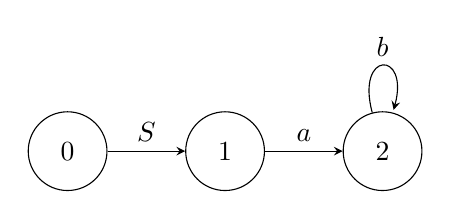
\begin{tikzpicture}[node distance=2cm, >=stealth, scale=1, transform shape]
            \tikzstyle{state}=[circle, draw, minimum size=1cm]

            % Stati
            \node[state] (q0) {0};
            \node[state, right of=q0] (q1) {1};
            \node[state, right of=q1] (q2) {2};

            % Frecce
            \draw[->] (q0) -- node[above] {\( S \)} (q1);
            \draw[->] (q1) -- node[above] {\( a \)} (q2);
            \draw[->] (q2) edge[loop above] node {\( b \)} (q2);
        \end{tikzpicture}
    \end{center}

    La tabella LR(0) mostra un conflitto \textit{shift-reduce}:

    \begin{center}
        \begin{tabular}{|c|c|c|c|c|}
        \hline
            & \( a \) & \( b \) & \( \$ \) & \( S \) \\
        \hline
            0   & S1 &     &     & g3  \\
            1   & r2/S2 & S2  & r2  &     \\
            2   & r3 & r3 & acc &     \\
            3   &     &     &     &     \\
        \hline
        \end{tabular}
    \end{center}

    Come risolvere il conflitto? 
    Usiamo il \textbf{lookahead}: guardiamo l'insieme \textit{Follow(S)}. Se il simbolo attuale appartiene a \( \text{Follow}(S) \), il conflitto è reale, altrimenti no!
    \\

    \textbf{Follow(S):}
    \[
        \text{Follow}(S) = \{ \$ \}
    \]

    \textbf{Risultato:}
    Risolvendo il conflitto a favore dello shift, otteniamo la seguente tabella SLR(1):

    \begin{center}
        \begin{tabular}{|c|c|c|c|c|}
        \hline
            & \( a \) & \( b \) & \( \$ \) & \( S \) \\
        \hline
            0   & S1 &     &     & g3  \\
            1   & S2 & r2  & r2  &     \\
            2   & r3 & r3 & acc &     \\
            3   &     &     &     &     \\
        \hline
        \end{tabular}
    \end{center}

    \textit{Conclusione:}  
    La grammatica \( G \) non è LR(0), ma è SLR(1) usando il lookahead per risolvere il conflitto
}

Il termine $SLR(1)$ sta per "Single, left-to-right, rightmost derivation” con un simbolo di lookahead

\nt{
    Se \( G \) ha produzioni \( \varepsilon \), allora \( G \) difficilmente è LR(0)  
    (caso banale in cui uno stato con item \( A \rightarrow \varepsilon \) non ha item del tipo \( B \rightarrow a \alpha \beta \))
}

\nt{
    Se \( L \) è libero deterministico e gode della \textbf{prefix-property}  
    (\emph{``\( L \) gode della prefix-property''}):  
    se \(\forall x, y \in L\) tale che \( x \) è prefisso di \( y \),  
    allora \( L \in \text{LR(0)} \)
    \vspace{0.3cm}
    \noindent Quindi, se \( L \) è libero deterministico ma non è LR(0),  
    allora \( L \) non gode della prefix-property.
}
\nt{
    Se \( L \in \text{LR(0)} \) ed è \textbf{finito}, allora gode della prefix-property.  
    Ovvero, se \( L \) è finito e non gode della prefix-property,  
    \[
    \text{allora } L \notin \text{LR(0)}.
    \]
}
\nt{
    Se \( L \in \text{LR(0)} \) ma è \textbf{infinito},  
    può \( L = \{a, ab\} \) non godere della prefix-property.
}

\subsection{Parser LR(1)}

Vi sono tuttavia delle grammatiche in cui neanche il look-ahead non basta, infatti il follow del non terminale in testa alla produzione è anch'esso troppo poco restrittivo

\esempio{
    \includegraphics[width=10cm]{esempio-lr-1.png}
}

Ed ecco che entrano in gioco i cosidetti \textbf{Parser LR(1)} che sfruttano gli $item LR(1)$
\subsubsection{Item LR(1)}
\dfn{Item LR(1)}{
    Un itwm $LR(1)$ è una coppia formata da:
    \begin{itemize}
        \item un item LR(0) che viene chiamato nucleo
        \item un simbolo di look-ahead in $T\cup\{\$\}$
    \end{itemize}
}
introdurre questo simbolo di look-ahead è fondamentale, così che si può decidere che azione fare in base al simbolo letto in input 
\esempio{
    Un possibile item $LR(1)$ è:
    \[
        [S\to V.= E, \$]   
    \]
    Dove abbiamo che $S\to V. = E$ è il cuore e $\$$ è il simbolo di look ahead. Se avessi uno stato con due item dentro:
    %! ERRORE GRAFICO, CHE CAZZ È? 
    \[
        \begin{array}{l}
            \lbrack S \to V \cdot E, \, \$\rbrack \\
            \lbrack S \to V \cdot, \, \$\rbrack
        \end{array}
    \]
    In questo caso se leggo il simbolo "=" si avrà uno shift per poi andare in un altro stato grazie al primo item, mentre se si legge $\$$ input avremo un reduce $E\to V$ proprio grazie al simbolo $\$$ di look-ahead
}

\paragraph{Intuizione}: se l'automa canonico $LR(1)$ è in uno stato che contiene l'item $LR(1)\quad [A\to\alpha.\beta,x]$:

\begin{itemize}
    \item $[A\to\alpha.\beta,x]$:
    \begin{itemize}
        \item Sta cercando di riconoscere la maniglia $\alpha \beta$
        \item di essa, $\alpha$ è già sulla pila
        \item Sull'input si aspetta una stringa derivabile da $\beta x$, ovvero si aspetta in input $\beta$ (per fare uno shift) ed un $x$ per la reduce
    \end{itemize}
    \item $[A\to\alpha.,x]$: fai la reduce $A\to \alpha$ se il prossimo input è proprio $x$
\end{itemize}
\subsubsection{NFA LR(1)}

Per creare gli NFA LR(1) si procede in maniera molto simile per NFA LR(0), ma tenendo traccia anche del simbolo di look ahead
\begin{itemize}
    \item Stati: sono item $LR(1)$ della grammatica aumentata
    \item $[S'\to.S, \$]$ è lo stato iniziale
    \item dallo stato $[ato\alpha.X\beta,a]$ c'è una transizione allo stato $[A\to \alpha X.\beta,a]$ etichettata $X$ per $X\in T\cup NT$
    \item dallo stato $[ato\alpha.X\beta,a]$ per $X\in T\cup NT$ e $\forall X\to\gamma$, c'è una $\epsilon$-transizione verso lo stato $\forall b\in First(\beta a).[X\to .\gamma, b]$, dove $First(\beta a)\subseteq T\cup\{\$\}$
\end{itemize}

\subsubsection{Adesso si passa ai DFA LR(0)}

Introduciamo le due funzioni ausiliarie: \textbf{Clos(I) e Goto(I,X)}

\begin{algorithm}
    \caption{Clos}
    \KwIn{I}
    \KwOut{I}

    \While{$I$ non è più modificato}{
        \ForEach{item $[A\to\alpha.X\beta]\in I$}{
            \ForEach{produzione $X\to \gamma$}{
                \ForEach{$b\in First(\beta a)$}{
                    aggiungi $[X\to .\gamma, b]$ ad $I$\;
                }
            }
        }
    }
    \Return $I$\;
\end{algorithm}

\begin{algorithm}
    \caption{Goto}
    \KwIn{I}
    \KwOut{I}

    Inizializza $J=\emptyset$\;
    \ForEach{item $[A\to\alpha.X\beta,a]\in I$}{
        aggiungi $[A\to \alpha X.\beta, a]$ a $J$\;
    }
    \Return $clos(J)$\;
\end{algorithm}
%! altro errore grafico. EH?

Viene presentato, qui, un esempio del grosso automa $LR(1)$
\esempio{
    Sia $G$ la seguente grammatica
    \[
        G = \begin{array}{l}
            0) S'\to S\\
            1) S\to CC\\
            2) C\to cC\\
            3) C\to d
        \end{array}
    \]

    Allora l'automa canonico LR(1) è:
    \begin{center}
    \includegraphics[width=10cm]{giga-automa.png}
    \end{center}
}

\subsubsection{Tabella di parsing $LR(0)$}
Uguale a quella $LR(0)$ e $SLR(1)$ solo che inserisco la reduce solo per il simbolo di look ahead. Riporto comunque la \textit{minghia} di descrizione riportata dal buon Babbo Natale

\begin{enumerate}
    \item Se \( x \in T \) e \( s \xrightarrow{x} t \) nell'automa LR(1), inserisco shift \( t \) in \( M[s, x] \).
    \item Se \([A \to \alpha \cdot, x] \in s\) e \( A 3\neq S' \), inserisco reduce \( A \to \alpha \) in \( M[s, x] \) \textit{(solo per \( x \) del look-ahead!)}.
    \item Se \([S' \to S \cdot, \$] \in s\), inserisco Accept in \( M[s, \$] \).
    \item Se \( A \in NT \) e \( s \xrightarrow{A} t \) nell'automa LR(1), inserisco goto \( t \) in \( M[s, A] \).
\end{enumerate}
\dfn{Grammatica di classe $LR(1)$}{
    Una grammatica libera $G$ e di classe $LR(1)$ se ogni casella della sua tabella di parsing $LR(1)$ contiene al massimo una azione
}

\esempio{
    Si consideri l'automa dell'esempio precedente, allora si ha:

    \includegraphics[width=10cm]{parsing-lr-0.png}

    si noti che per questa grammatica la tabella di parsing ha 7 stati anzichè 10, ed è pure senza conflitti 
}

\subsection{Parser $LALR(1)$}

Il problema coi parser $LR(1)$ è che le tabelle sue tabelle di parsing sono molto grandi (centinaia di migliaia di stati per linguaggi di media grandezza), pertanto entrano in gioco i $LALR(1)$ che rappresentano un buon compromesso tra semplicità e selettività

\subsubsection{Come si ottiene il parser $LALR(1)$}


Si osservi che:
\begin{enumerate}
    \item \textbf{Nucleo di uno stato LR(1)}: \\
    L'insieme di item LR(0) ottenuto dimenticando i \textit{look-ahead} dagli item LR(1).
    
    \item \textbf{Nucleo di stato LR(1)}: \\
    Ogni nucleo di uno stato LR(1) corrisponde a uno stato dell'automa LR(0).
    
    \item \textbf{Transizioni dell'automa LR(1)}: \\
    Le transizioni dell'automa LR(1) dipendono solo dal nucleo. La funzione \( \text{goto}(I, X) \) usa di \( I \) solo le parti ``nucleo/LR(0)'' degli item LR(1).
\end{enumerate}

\subsubsection{Tabella di parsing LALR(1)}
La tabella di parsing LALR(1) si ottiene da quella LR(1) \textbf{fondendo insieme gli stati con lo stesso nucleo}. \\
Ciò comporta:
\begin{itemize}
    \item \textbf{Meno righe}, poiché gli stati dell'automa LR(0) vengono combinati.
    \item \textbf{Meno reduce} rispetto alla tabella SLR(1).
\end{itemize}

\esempio{
    Sia la grammatica degli esempi precedenti, ecco qui il nostro automa
    \begin{center}
    \includegraphics[width=10cm]{parsing-lalr-1.png}
    \end{center}
}

\subsubsection{Passando da lr(1) a LALR(1)}

La fusione di due stati $LR(1)$ con lo stesso core può causare conflitti

\thm{Babbo natale Theorem}{
    Quando fondo due stati $LR(1)$ per generare un parser $LALR(1)$ sono possibili solo conflitti \textbf{reduce/reduce}
}
\dimostrazione{
    Supponiamo che in $s$, stato ottenuto dalla fusione di due stati $LR(1)$, $s_1$ ed $s_2$

    Allora in $s$ esiste un item $[S\to\alpha.a]$ e un item $[B\to\beta.a\gamma, b]$ (H1)

    Suppongo che $[A\to\alpha.,a]\in s_1$ (H2)

    per (H1) $[A\to\alpha., a]\in s_1$ e $[B\to\beta.a\gamma,c]\in s_1$ (H3) dato che se ho fuso insieme $s_1$ ed $s_2$ allora il core $[B\to\beta.a\gamma]$ deve per forza esserci in entrambi $\heartsuit$

    Per (H3) si ha che anche in $LR(1)$ si verificherebbe un conflitto shift-reduce, contro l'ipotesi che la tabella $lr(1)$ non presenti conflitti, pertanto se $LR(1)$ è senza conflitti, $LARL(1)$ potrebbe solo presentare conflitti reduce-reduce
}

\nt{
    Se si generano conflitti, allora $G$ non è $LALR(1)$, pur essendo $LR(1)$
}

\esempio{
    \includegraphics[width=10cm]{ultimo-lalr-1.png}
}

\section{Grammatiche $LR(k)$}
Ci si può concentrare adesso alle grammatiche $LR$ con $k$ simboli di look-ahead, nessuno le usa perché molto confusionarie e macchinose, ma si possono andare a definire

Prima della definizione di grammatica occorre definire \textbf{gli item $LR(k)$}

\dfn{
    Item $LR(k)$
}{
    Si definisce un \textbf{item $LR(k)$}, un item formato da una coppia formata da un item $LR(0)$ e una stringa $\beta$ la cui lunghezza è inferiore a $k$, e si denota nel seguente modo:
    \[
        [item\;LR(0), \beta] \text{ con }|\beta|\leq k
    \]
}

Tali item hanno queste caratteristiche:
\begin{itemize}
    \item Lo stato iniziale è sempre $[S'\to.S, \$]$
    \item Sia $s$ uno stato dell'automa canonico $LR(k)$, si che $([A\to \alpha.X\gamma, \beta]\in s\land \exists \text{ la produzione }X\to \gamma\land w\in First_k(\gamma\beta ) ) \implies [X\to.\gamma ,w]\in s$ 
\end{itemize}

Si può subito intuire che un automa canonico $LR(k)$ genera una quantità molto grande di stati molto difficili da gestire a mano

Una volta costruito l'automa canonico $LR(k)$ si passa alla tabella di parsing $LR(k)$ con collonne su $T^k$ (cioè su stringhe di terminali lunghe $k$)

\dfn{Grammatica $LR(k)$}{
    Si definisce $G$ una grammatica $LR(k)$ una grammatica costruita a partire da una tabella di parsing $LR(k)$, ottenuta a partire dall'automa canonico $LR(k)$, con le seguenti caratteristiche:
    \begin{itemize}
        \item Contiene al più un'azioni per ogni entrata della tabella
        \item non esistono sue $w_1$ e $w_2$ sulle colonne tali che $w_1$ è prefisso di $w_2$ e per almeno una righe le 2 corrispondenti entrate contengono un'azione
    \end{itemize}
}

\nt{Ovviamente la tabella viene tiempita nel modo ovvio per le azioni di shift/accept, mentre le reduce sono messe solo in corrispondenza del lookahead, ad esempio $[A\to\alpha.,w]$}

\subsection{Grammatiche $SLR(k)$}

Si parte dell'automa canonico $LR(0)$ e si riempie la tabella di parsing $SLR(k)$ - che ha colonne su $T^k$ - secondo la seguente legge: 
\[
    ([A\to\alpha.]\in s\land A\neq S')\implies \forall w\in Follow_k(A).(M[s,w]=\text{ reduce } A\to\alpha)
\] 

\subsection{
    Grammatiche $LALR(k)$
}
Si parte dall'automa canonico $LR(k)$ e si fondono insieme due stato con lo stesso nucleo, se non vi sono conflitti $G$ è $LALR(k)$

\subsection{relazione tra le varie grammatiche}
Si può noti il seguente schema riassuntivo:
\begin{center}
    \includegraphics[width=10cm]{inclusione-tra-grammatiche.png}
\end{center}

Si può concludere che:
\[
LR:
\begin{cases}
    \text{SLR}(k) \subset \text{LALR}(k) \subset \text{LR}(k) & \text{per ogni } k \geq 1 \\
    \text{SLR}(1) \subset \text{SLR}(2) \subset \dots \subset \text{SLR}(k) \\
    \text{LALR}(1) \subset \text{LALR}(2) \subset \dots \subset \text{LALR}(k) \\
    \text{LR}(0) \subset \text{LR}(1) \subset \dots \subset \text{LR}(k)
\end{cases}
\]

\textbf{LL vs LR:}
\[
LL vs LR:
\begin{cases}
    \text{LL}(k) \subset \text{LR}(k) & \text{per ogni } k \geq 0 \\
    \text{LL}(k) \not\subset \text{LR}(k-1) & \text{per ogni } k \geq 1
\end{cases}
\]

\mprop{}{
    \begin{itemize}
        \item Se $G$ è $LL(k)$, allora $G$ è non ambigua e $L(G)$ è deterministico
        \item Se $G$ è $LR(k)$, allora $G$ è non ambigua e $L(G)$ è deterministico
    \end{itemize}
}
\nt{
    Esistono linguaggi generati da grammatiche non ambigue, ma nondeterministici
}

\esempio{
    Sia $G$ la seguente grammatica:
    \[
        S\to aSa\mid bSb\mid\epsilon      
    \]
    Allora
    \[
        L(G) = \{ww^R\mid w\in\{a,b\}^*\}
    \]
}

\section{Linguaggi generati dalle varie grammatiche}
\dfn{
    Linguaggio di classe $X$
}{
    Un linguaggio $L$ si definisce di classe $X$ se $\exists G$ di classe $X$ tale che $L=L(G)$

    Dove $X$ sta per $LR(0)/SLR(1)/LL(1)/\dots$
}
Se classifichiamo i linguaggi anziché le grammatica, il diagramma si semplifica molto

\esempio{
    \begin{center}
    \includegraphics[width=10cm]{esempio-linguaggio.png}
    \end{center}
}
Si considerino queste note

\nt{
    Un linguaggio è libero deterministico se è accettato, per stato dinale 
}
\nt{
    Ogni linguaggio regolare è generato da una grammatica di classe $LL(1)$
}
\nt{
    esistono linguaggi regolari che non sono $LR(0)$ 

    Ad es. $L=\{a,ab\}$
}
Si considerino i seguenti teoremi:
\teorema{
    Un linguaggio è libero deterministico sse è generato da una grammatica $LR(1)$ per qualche $k\geq 0$
}
\teorema{
    Un linguaggio è libero deterministico sse è generato da una grammatica $SLR(1)$
}
\teorema{
    I linguaggi generati da grammatica $LL(k)$ sono esattamente contenuti nei linguaggi generati da grammatiche $SLR(1),\forall k\geq 0$
}
\subsubsection{calssificazione dei linguaggi}
Si noti il seguente schema:
\begin{center}
    \includegraphics[width=10cm]{classificazione-dei-linguaggi.png}
\end{center}
\nt{
    Se $G$ è $LR(k)$, esiste $G'\in SLR(1)$ quivalente, ma $G'$ può essere molto più complessa di $G$ 
}

\esempio{
    Sia $L=\{a^i b^j\mid i\geq j\geq 0\}$ libero deterministico

    Si può notare che
    \begin{center}
        \begin{tikzpicture}
            \node[state, initial] (q) {$q_0$};
            \node[state, right of=q] (q1) {$q_1$};
            
            \path[->] 
                    (q_0) edge [loop above] node {$a, X/aX$} ()
                        edge  node {$b,a/\epsilon$} (q1)
                    (q_1) edge [loop above]  node {$b,a/\epsilon$} ();
        \end{tikzpicture}  
    \end{center}
    è il DPDA che riconosce $L$ per stato finale

    $L$ però non è $LL(k)$ per nessun $k$, tuttavia $L$ è $SLR(1)$, infatti esiste $G$ $SLR(1)$ tale che $L(G)=L$:
    \[
        \begin{array}{l}
            S\to aS\mid B\\
            B\to aBb\mid \epsilon
        \end{array}
    \]
    \begin{center}
    \includegraphics[width=10cm]{automa-bellino.png}
    \end{center}

    La cui tabella di parsing è:
    \[
        \begin{array}{c|c|c|c|c|c}
        & a & b & \$ & S & B \\
        \hline
        0 & S_3 & R_4 & R_4 & G_1 & G_2 \\
        1 & & & \text{acc} & & \\
        2 & & & R_2 & & \\
        3 & S_3 & R_4 & & G_4 & G_5 \\
        4 & & & R_4 & & \\
        5 & S_3 & & R_2 & & \\
        6 & R_3 & R_3 & & &
        \end{array}
    \]

    \textit{Tabella di parsing SLR(1) senza conflitti} \\
    $\Rightarrow G$ è SLR(1)
}

\nt{
    \begin{enumerate}
        \item $L_1 = \{ a^n b^n \mid n \geq 1 \} \in \text{LL}(1) \in \text{LR}(0)$ \\
            $L_2 = \{ a^n c^m \mid n, m \geq 1 \} \in \text{LL}(1) \in \text{LR}(0)$ \\
            
            ma $L_1 \cup L_2$ non è $\text{LL}(k)$ per nessun $k$, \\
            mentre $L_1 \cup L_2 \in \text{LR}(0)$ \\
            $\Rightarrow$ l'unione di linguaggi $\text{LL}(1)$ può non essere $\text{LL}(1)$
        \item $L_1 = \{ a \} \in \text{LL}(1) \in \text{LR}(0)$ \\
            $L_2 = \{ a b \} \in \text{LL}(1) \in \text{LR}(0)$ \\
            
            ma $L_1 \cup L_2$ non è $\text{LR}(0)$ perché non gode della prefix-property, \\
            mentre $L_1 \cup L_2 \in \text{LL}(1)$ \\
            $\Rightarrow$ l'unione di linguaggi $\text{LR}(0)$ può non essere $\text{LR}(0)$
        \item $L_1 = a^* = \{ a^n \mid n \geq 0 \} \in \text{LL}(1)$ \\
            $L_2 = \{ a^n b^n \mid n \geq 0 \} \in \text{LL}(1)$ \\
            
            ma $L_1 \cdot L_2 = \{ a^i b^j \mid i \geq j \geq 0 \}$ non è $\text{LL}(k)$ per nessun $k$ \\
            $\Rightarrow$ la concatenazione di due linguaggi $\text{LL}(1)$ può non essere $\text{LL}(1)$
    \end{enumerate}
}
